\begin{frame}
    \frametitle{Bare metal vs RTOS}
    \includegraphics[scale=0.2]{RTOS_werking.png}
    bron foto: academy.nordicsemi.com
\end{frame}

\begin{frame}
    \frametitle{Bare metal vs RTOS}
    Bare-metal
    Voordelen:
    \begin{itemize}
        \item meer efficient
        \item minder geheugen
        \item kan sneller werken
    \end{itemize}
    \vspace{0.5cm}
    Nadelen:
    \begin{itemize}
        \item complexere architectuur
        \item werkt op een type microcontroller
        \item door complexiteit kan minder snel zijn dan RTOS
    \end{itemize}
    \vspace{0.5cm}
    Beiden hebben ISR's.
\end{frame}


\begin{frame}
    \frametitle{Referentiespanning}
    
    \only<1>{
        \begin{figure}
            \centering
            \includegraphics[width=\textwidth]{referenceBlock.pdf}
        \end{figure}
    }

    \only<2>{
        \begin{figure}
            \centering
            \def\svgwidth{0.6\textwidth}
            \subsection{Spanningsreferentie}\label{sec:referenceVoltage}

De ISFET uitleesschakeling heeft een spanningsreferentie nodig om te werken. Deze spanningsreferentie kan op meerdere manieren gegenereerd worden.
% TODO: Vertel misschien over andere methoden.
Uiteindelijk is er een spanningsdeler gekozen om de spanningsreferentie mee te implementeren. De schakeling van deze spanningsdeler is te zien in \autoref{fig:divider}.
De condensator wordt gebruikt om ruis te verminderen op hogere frequenties, en dient ook als filter voor hoogfrequente fouten in de voedingsspanning.

\begin{figure}[ht]
    \centering
    \def\svgwidth{0.5\textwidth}
    \subsection{Spanningsreferentie}\label{sec:referenceVoltage}

De ISFET uitleesschakeling heeft een spanningsreferentie nodig om te werken. Deze spanningsreferentie kan op meerdere manieren gegenereerd worden.
% TODO: Vertel misschien over andere methoden.
Uiteindelijk is er een spanningsdeler gekozen om de spanningsreferentie mee te implementeren. De schakeling van deze spanningsdeler is te zien in \autoref{fig:divider}.
De condensator wordt gebruikt om ruis te verminderen op hogere frequenties, en dient ook als filter voor hoogfrequente fouten in de voedingsspanning.

\begin{figure}[ht]
    \centering
    \def\svgwidth{0.5\textwidth}
    \subsection{Spanningsreferentie}\label{sec:referenceVoltage}

De ISFET uitleesschakeling heeft een spanningsreferentie nodig om te werken. Deze spanningsreferentie kan op meerdere manieren gegenereerd worden.
% TODO: Vertel misschien over andere methoden.
Uiteindelijk is er een spanningsdeler gekozen om de spanningsreferentie mee te implementeren. De schakeling van deze spanningsdeler is te zien in \autoref{fig:divider}.
De condensator wordt gebruikt om ruis te verminderen op hogere frequenties, en dient ook als filter voor hoogfrequente fouten in de voedingsspanning.

\begin{figure}[ht]
    \centering
    \def\svgwidth{0.5\textwidth}
    \input{img/divider.pdf_tex}
    \caption{De schakeling van de spanningsdeler die dient als spanningsreferentie.}
    \label{fig:divider}
\end{figure}

\noindent
De overdracht van deze spanningsdeler is te vinden in \autoref{eq:dividerTransfer}.
\begin{equation}\label{eq:dividerTransfer}
    H(s) = \frac{U_{ref}(s)}{U_{dd}(s)} = \frac{R_2}{R_1 + R_2 + R_2Cs}
\end{equation}

\noindent
Het vermogen dat de spanningsdeler dissipeert, kan met \autoref{eq:dividerPower} berekend worden.
\begin{equation}\label{eq:dividerPower}
    P(s) = U_{dd}(s)^2\frac{1+R_2Cs}{R_1 + R_2 + R_1R_2Cs}
\end{equation}
Met een constante DC ingangsspanning kan dit vereenvoudigd worden naar \autoref{eq:dividerPowerSimple}.
\begin{equation}\label{eq:dividerPowerSimple}
    P = \frac{U_{dd}^2}{R_1 + R_2}
\end{equation}

\noindent
Om de ruis van deze schakeling te berekenen moet een aantal stappen genomen worden. Aangezien de ingangsbron $U_{dd}$ een spanningsbron is, kan deze als kortsluiting genomen worden. Op deze manier kunnen de twee weerstanden parallel genomen worden, en verandert de schakeling in een simpel RC filter. In \autoref{fig:dividerNoise} is deze omgebouwde schakeling te zien.

\begin{figure}[ht]
    \centering
    \def\svgwidth{0.35\textwidth}
    \input{img/dividerNoise.pdf_tex}
    \caption{De omgebouwde schakeling om ruis mee te berekenen.}
    \label{fig:dividerNoise}
\end{figure}

\noindent
Voor de spectrale spanningsruisdichtheid aan de uitgang $U_{ref}$ kan \autoref{eq:dividerNoiseLaplace} worden opgesteld.
\begin{equation}\label{eq:dividerNoiseLaplace}
    S_{n,u_{ref}} = 4kTR_e\left(\frac{1}{1 + R_eCs}\right)^2
\end{equation}
Wanneer de absolute waarde van de ruis wordt genomen, kan deze over de bandbreedte geïntegreerd worden. Dit resulteert in \autoref{eq:dividerNoiseInt}.
\begin{equation}\label{eq:dividerNoiseInt}
    u_{n,ref}^2 = \int_{\omega_l}^{\omega_h} 4kTR_e\left(\frac{1}{\sqrt{1 + (R_eC\omega)^2}}\right)^2 d\omega
\end{equation}
Het integraal van deze formule komt uit op \autoref{eq:dividerNoiseIntegrated}.
\begin{equation}\label{eq:dividerNoiseIntegrated}
    u_{n,ref}^2 = \frac{4kT}{C}\left[\arctan(R_eC\omega_h) - \arctan(R_eC\omega_l)\right]
\end{equation}

Zolang de spanning stabiel is hoeft de referentie geen exact gedefinieerde spanning te hebben. Dit is omdat de ADC die de waarde van de sensor gaat uitlezen deze referentiespanning ook als referentie zal gebruiken. De waarde moet echter ergens rond de 1.1V zitten, om de stroombron te laten werken.
In \autoref{sec:currentSource} is hier meer over te lezen.
Aangezien de ingangsspanning 1.8V is, zal de DC overdracht $1.1 / 1.8 = \frac{11}{18}$ zijn. Hieruit komt de weerstandsverhouding in \autoref{eq:dividerResistors}.
\begin{equation}\label{eq:dividerResistors}
    \frac{R_1}{R_2} = \frac{7}{11}
\end{equation}
Een hogere $R_1$ zorgt voor een lager vermogensverbruik, maar ook een hogere ruis. Dit is te zien in \autoref{fig:dividerPlots}.

\begin{figure}
    \centering
    \begin{subfigure}[b]{0.45\textwidth}
        \centering
        \input{plots/dividerNoise}
        \caption{Spanningsruis}
        \label{fig:dividerNoisePlot}
    \end{subfigure}
    \hfill
    \begin{subfigure}[b]{0.45\textwidth}
        \centering
        \input{plots/dividerPower}
        \caption{Vermogensverbruik}
        \label{fig:dividerPower}
    \end{subfigure}
    \caption{De ruis en het vermogensverbruik van de spanningsdeler, ten opzichte van de gekozen weerstandswaarde $R_1$.}
    \label{fig:dividerPlots}
\end{figure}
Op $R_1 = 1\si{\mega\ohm}$ en $C = 10\si{\micro\farad}$ is de spanningsruis $u_{n,ref} = 51\si{\nano\volt}$ en het vermogensverbruik $P = 1.3\si{\micro\watt}$. De andere weerstandswaarde is dan $R_2 \approx 1.6 \si{\mega\ohm}$. Deze waardes vallen binnen de specificaties.

[WELKE SPECS??]
    \caption{De schakeling van de spanningsdeler die dient als spanningsreferentie.}
    \label{fig:divider}
\end{figure}

\noindent
De overdracht van deze spanningsdeler is te vinden in \autoref{eq:dividerTransfer}.
\begin{equation}\label{eq:dividerTransfer}
    H(s) = \frac{U_{ref}(s)}{U_{dd}(s)} = \frac{R_2}{R_1 + R_2 + R_2Cs}
\end{equation}

\noindent
Het vermogen dat de spanningsdeler dissipeert, kan met \autoref{eq:dividerPower} berekend worden.
\begin{equation}\label{eq:dividerPower}
    P(s) = U_{dd}(s)^2\frac{1+R_2Cs}{R_1 + R_2 + R_1R_2Cs}
\end{equation}
Met een constante DC ingangsspanning kan dit vereenvoudigd worden naar \autoref{eq:dividerPowerSimple}.
\begin{equation}\label{eq:dividerPowerSimple}
    P = \frac{U_{dd}^2}{R_1 + R_2}
\end{equation}

\noindent
Om de ruis van deze schakeling te berekenen moet een aantal stappen genomen worden. Aangezien de ingangsbron $U_{dd}$ een spanningsbron is, kan deze als kortsluiting genomen worden. Op deze manier kunnen de twee weerstanden parallel genomen worden, en verandert de schakeling in een simpel RC filter. In \autoref{fig:dividerNoise} is deze omgebouwde schakeling te zien.

\begin{figure}[ht]
    \centering
    \def\svgwidth{0.35\textwidth}
    \begin{tikzpicture}
    \pgfplotsset{width=\textwidth}
    \newcommand\BOLZ{1.380649e-23}
    \newcommand\TEMP{300}
    \newcommand\OMEGAC{15*2*pi}
    \newcommand\RESRAT{(7/11)}
    \newcommand\REQU{(1/(1/x + \RESRAT/x))}
    \newcommand\CAP{0.000001}

    \pgfplotsset{set layers}
    \begin{axis}[
        xmode=log,
        ymode=log,
        xlabel={$R_1 [\si{\ohm}]$},
        ylabel={$u_{n,out} [\si{\volt}]$},
        xmin=1e3, xmax=1e7,
        grid=major
    ]

    \addplot [
        red,
        domain=1e3:1e7,
        samples=201
    ]
    {sqrt((4 * \BOLZ * \TEMP / \CAP) * rad(atan(\REQU * \CAP * \OMEGAC)))};
    \end{axis}
\end{tikzpicture}
    \caption{De omgebouwde schakeling om ruis mee te berekenen.}
    \label{fig:dividerNoise}
\end{figure}

\noindent
Voor de spectrale spanningsruisdichtheid aan de uitgang $U_{ref}$ kan \autoref{eq:dividerNoiseLaplace} worden opgesteld.
\begin{equation}\label{eq:dividerNoiseLaplace}
    S_{n,u_{ref}} = 4kTR_e\left(\frac{1}{1 + R_eCs}\right)^2
\end{equation}
Wanneer de absolute waarde van de ruis wordt genomen, kan deze over de bandbreedte geïntegreerd worden. Dit resulteert in \autoref{eq:dividerNoiseInt}.
\begin{equation}\label{eq:dividerNoiseInt}
    u_{n,ref}^2 = \int_{\omega_l}^{\omega_h} 4kTR_e\left(\frac{1}{\sqrt{1 + (R_eC\omega)^2}}\right)^2 d\omega
\end{equation}
Het integraal van deze formule komt uit op \autoref{eq:dividerNoiseIntegrated}.
\begin{equation}\label{eq:dividerNoiseIntegrated}
    u_{n,ref}^2 = \frac{4kT}{C}\left[\arctan(R_eC\omega_h) - \arctan(R_eC\omega_l)\right]
\end{equation}

Zolang de spanning stabiel is hoeft de referentie geen exact gedefinieerde spanning te hebben. Dit is omdat de ADC die de waarde van de sensor gaat uitlezen deze referentiespanning ook als referentie zal gebruiken. De waarde moet echter ergens rond de 1.1V zitten, om de stroombron te laten werken.
In \autoref{sec:currentSource} is hier meer over te lezen.
Aangezien de ingangsspanning 1.8V is, zal de DC overdracht $1.1 / 1.8 = \frac{11}{18}$ zijn. Hieruit komt de weerstandsverhouding in \autoref{eq:dividerResistors}.
\begin{equation}\label{eq:dividerResistors}
    \frac{R_1}{R_2} = \frac{7}{11}
\end{equation}
Een hogere $R_1$ zorgt voor een lager vermogensverbruik, maar ook een hogere ruis. Dit is te zien in \autoref{fig:dividerPlots}.

\begin{figure}
    \centering
    \begin{subfigure}[b]{0.45\textwidth}
        \centering
        \begin{tikzpicture}
    \pgfplotsset{width=\textwidth}
    \newcommand\BOLZ{1.380649e-23}
    \newcommand\TEMP{300}
    \newcommand\OMEGAC{15*2*pi}
    \newcommand\RESRAT{(7/11)}
    \newcommand\REQU{(1/(1/x + \RESRAT/x))}
    \newcommand\CAP{0.000001}

    \pgfplotsset{set layers}
    \begin{axis}[
        xmode=log,
        ymode=log,
        xlabel={$R_1 [\si{\ohm}]$},
        ylabel={$u_{n,out} [\si{\volt}]$},
        xmin=1e3, xmax=1e7,
        grid=major
    ]

    \addplot [
        red,
        domain=1e3:1e7,
        samples=201
    ]
    {sqrt((4 * \BOLZ * \TEMP / \CAP) * rad(atan(\REQU * \CAP * \OMEGAC)))};
    \end{axis}
\end{tikzpicture}
        \caption{Spanningsruis}
        \label{fig:dividerNoisePlot}
    \end{subfigure}
    \hfill
    \begin{subfigure}[b]{0.45\textwidth}
        \centering
        \begin{tikzpicture}
    \pgfplotsset{width=\textwidth}
    \newcommand\OMEGAC{10*2*pi}
    \newcommand\RESRAT{(7/11)}

    \begin{axis}[
        xmode=log,
        ymode=log,
        xlabel={$R_1 [\si{\ohm}]$},
        ylabel={$P [\si{\watt}]$},
        xmin=1e3, xmax=2e6,
        grid=major
    ]

    \addplot [
        blue,
        domain=1e3:2e6,
        samples=201
    ]
    {1.8 / (x + x/\RESRAT)};
    \end{axis}
\end{tikzpicture}
        \caption{Vermogensverbruik}
        \label{fig:dividerPower}
    \end{subfigure}
    \caption{De ruis en het vermogensverbruik van de spanningsdeler, ten opzichte van de gekozen weerstandswaarde $R_1$.}
    \label{fig:dividerPlots}
\end{figure}
Op $R_1 = 1\si{\mega\ohm}$ en $C = 10\si{\micro\farad}$ is de spanningsruis $u_{n,ref} = 51\si{\nano\volt}$ en het vermogensverbruik $P = 1.3\si{\micro\watt}$. De andere weerstandswaarde is dan $R_2 \approx 1.6 \si{\mega\ohm}$. Deze waardes vallen binnen de specificaties.

[WELKE SPECS??]
    \caption{De schakeling van de spanningsdeler die dient als spanningsreferentie.}
    \label{fig:divider}
\end{figure}

\noindent
De overdracht van deze spanningsdeler is te vinden in \autoref{eq:dividerTransfer}.
\begin{equation}\label{eq:dividerTransfer}
    H(s) = \frac{U_{ref}(s)}{U_{dd}(s)} = \frac{R_2}{R_1 + R_2 + R_2Cs}
\end{equation}

\noindent
Het vermogen dat de spanningsdeler dissipeert, kan met \autoref{eq:dividerPower} berekend worden.
\begin{equation}\label{eq:dividerPower}
    P(s) = U_{dd}(s)^2\frac{1+R_2Cs}{R_1 + R_2 + R_1R_2Cs}
\end{equation}
Met een constante DC ingangsspanning kan dit vereenvoudigd worden naar \autoref{eq:dividerPowerSimple}.
\begin{equation}\label{eq:dividerPowerSimple}
    P = \frac{U_{dd}^2}{R_1 + R_2}
\end{equation}

\noindent
Om de ruis van deze schakeling te berekenen moet een aantal stappen genomen worden. Aangezien de ingangsbron $U_{dd}$ een spanningsbron is, kan deze als kortsluiting genomen worden. Op deze manier kunnen de twee weerstanden parallel genomen worden, en verandert de schakeling in een simpel RC filter. In \autoref{fig:dividerNoise} is deze omgebouwde schakeling te zien.

\begin{figure}[ht]
    \centering
    \def\svgwidth{0.35\textwidth}
    \begin{tikzpicture}
    \pgfplotsset{width=\textwidth}
    \newcommand\BOLZ{1.380649e-23}
    \newcommand\TEMP{300}
    \newcommand\OMEGAC{15*2*pi}
    \newcommand\RESRAT{(7/11)}
    \newcommand\REQU{(1/(1/x + \RESRAT/x))}
    \newcommand\CAP{0.000001}

    \pgfplotsset{set layers}
    \begin{axis}[
        xmode=log,
        ymode=log,
        xlabel={$R_1 [\si{\ohm}]$},
        ylabel={$u_{n,out} [\si{\volt}]$},
        xmin=1e3, xmax=1e7,
        grid=major
    ]

    \addplot [
        red,
        domain=1e3:1e7,
        samples=201
    ]
    {sqrt((4 * \BOLZ * \TEMP / \CAP) * rad(atan(\REQU * \CAP * \OMEGAC)))};
    \end{axis}
\end{tikzpicture}
    \caption{De omgebouwde schakeling om ruis mee te berekenen.}
    \label{fig:dividerNoise}
\end{figure}

\noindent
Voor de spectrale spanningsruisdichtheid aan de uitgang $U_{ref}$ kan \autoref{eq:dividerNoiseLaplace} worden opgesteld.
\begin{equation}\label{eq:dividerNoiseLaplace}
    S_{n,u_{ref}} = 4kTR_e\left(\frac{1}{1 + R_eCs}\right)^2
\end{equation}
Wanneer de absolute waarde van de ruis wordt genomen, kan deze over de bandbreedte geïntegreerd worden. Dit resulteert in \autoref{eq:dividerNoiseInt}.
\begin{equation}\label{eq:dividerNoiseInt}
    u_{n,ref}^2 = \int_{\omega_l}^{\omega_h} 4kTR_e\left(\frac{1}{\sqrt{1 + (R_eC\omega)^2}}\right)^2 d\omega
\end{equation}
Het integraal van deze formule komt uit op \autoref{eq:dividerNoiseIntegrated}.
\begin{equation}\label{eq:dividerNoiseIntegrated}
    u_{n,ref}^2 = \frac{4kT}{C}\left[\arctan(R_eC\omega_h) - \arctan(R_eC\omega_l)\right]
\end{equation}

Zolang de spanning stabiel is hoeft de referentie geen exact gedefinieerde spanning te hebben. Dit is omdat de ADC die de waarde van de sensor gaat uitlezen deze referentiespanning ook als referentie zal gebruiken. De waarde moet echter ergens rond de 1.1V zitten, om de stroombron te laten werken.
In \autoref{sec:currentSource} is hier meer over te lezen.
Aangezien de ingangsspanning 1.8V is, zal de DC overdracht $1.1 / 1.8 = \frac{11}{18}$ zijn. Hieruit komt de weerstandsverhouding in \autoref{eq:dividerResistors}.
\begin{equation}\label{eq:dividerResistors}
    \frac{R_1}{R_2} = \frac{7}{11}
\end{equation}
Een hogere $R_1$ zorgt voor een lager vermogensverbruik, maar ook een hogere ruis. Dit is te zien in \autoref{fig:dividerPlots}.

\begin{figure}
    \centering
    \begin{subfigure}[b]{0.45\textwidth}
        \centering
        \begin{tikzpicture}
    \pgfplotsset{width=\textwidth}
    \newcommand\BOLZ{1.380649e-23}
    \newcommand\TEMP{300}
    \newcommand\OMEGAC{15*2*pi}
    \newcommand\RESRAT{(7/11)}
    \newcommand\REQU{(1/(1/x + \RESRAT/x))}
    \newcommand\CAP{0.000001}

    \pgfplotsset{set layers}
    \begin{axis}[
        xmode=log,
        ymode=log,
        xlabel={$R_1 [\si{\ohm}]$},
        ylabel={$u_{n,out} [\si{\volt}]$},
        xmin=1e3, xmax=1e7,
        grid=major
    ]

    \addplot [
        red,
        domain=1e3:1e7,
        samples=201
    ]
    {sqrt((4 * \BOLZ * \TEMP / \CAP) * rad(atan(\REQU * \CAP * \OMEGAC)))};
    \end{axis}
\end{tikzpicture}
        \caption{Spanningsruis}
        \label{fig:dividerNoisePlot}
    \end{subfigure}
    \hfill
    \begin{subfigure}[b]{0.45\textwidth}
        \centering
        \begin{tikzpicture}
    \pgfplotsset{width=\textwidth}
    \newcommand\OMEGAC{10*2*pi}
    \newcommand\RESRAT{(7/11)}

    \begin{axis}[
        xmode=log,
        ymode=log,
        xlabel={$R_1 [\si{\ohm}]$},
        ylabel={$P [\si{\watt}]$},
        xmin=1e3, xmax=2e6,
        grid=major
    ]

    \addplot [
        blue,
        domain=1e3:2e6,
        samples=201
    ]
    {1.8 / (x + x/\RESRAT)};
    \end{axis}
\end{tikzpicture}
        \caption{Vermogensverbruik}
        \label{fig:dividerPower}
    \end{subfigure}
    \caption{De ruis en het vermogensverbruik van de spanningsdeler, ten opzichte van de gekozen weerstandswaarde $R_1$.}
    \label{fig:dividerPlots}
\end{figure}
Op $R_1 = 1\si{\mega\ohm}$ en $C = 10\si{\micro\farad}$ is de spanningsruis $u_{n,ref} = 51\si{\nano\volt}$ en het vermogensverbruik $P = 1.3\si{\micro\watt}$. De andere weerstandswaarde is dan $R_2 \approx 1.6 \si{\mega\ohm}$. Deze waardes vallen binnen de specificaties.

[WELKE SPECS??]
        \end{figure}
    }

\end{frame}


\begin{frame}
    \frametitle{Ruis analyse}

    \begin{figure}
        \centering
        \def\svgwidth{0.7\textwidth}
        \input{ISFETCircuitBestNoise.pdf_tex}
    \end{figure}
    \begin{equation*}\label{eq:measureNoiseOut}
        S_{u_{{n,out}}} = \left(S_{u_{{n,ref}}} + S_{u_{{n,n}}} + S_{i_{{n,in}}}\left(Z_{fet} // R\right)^2\right) \cdot H^2(ph)
    \end{equation*}

\end{frame}

\begin{frame}
    \frametitle{Power and harvest schema}
    \centering
    \includegraphics[scale=0.4]{powerAndHarvest2.pdf}
\end{frame}

\begin{frame}
    \frametitle{Efficiency buck only vs buck-boost}
    \centering
    \includegraphics[scale=0.9]{buckvsbuckboost.png}\\
    Efficiency gekozen mode, oranje lijn. Rond 90\%\\
    Bron: LTC3330 datasheet
\end{frame}

\begin{frame}
    \frametitle{Buck-boost swithcing}
    \centering
    \includegraphics[scale=0.9]{buck_boost_switching.png}\\
    Bron: LTC3330 datasheet
\end{frame}

\begin{frame}
    \frametitle{LDO Spanning}
    \centering
    \includegraphics[scale=0.9]{ldo_spannign.png}\\
    Bron: LTC3330 datasheet
\end{frame}

\begin{frame}
    \frametitle{Buck step respone}
    \centering
    \includegraphics[scale=0.9]{buck_step_response.png}\\
    Bron: LTC3330 datasheet
\end{frame}

\begin{frame}
    \frametitle{LDO step respone}
    \centering
    \includegraphics[scale=0.9]{ldo_step.png}\\
    Bron: LTC3330 datasheet
\end{frame}

\begin{frame}
    \frametitle{Sensor uitlees + analog}
    \centering
    \includegraphics[scale=0.3]{sensorBord.png}\\
\end{frame}

\begin{frame}
    \frametitle{Power and Harvest}
    \centering
    \includegraphics[scale=0.18]{powerAndHarvest.png}\\
\end{frame}

\begin{frame}
    \frametitle{Test Ugs Uds}
    \centering
    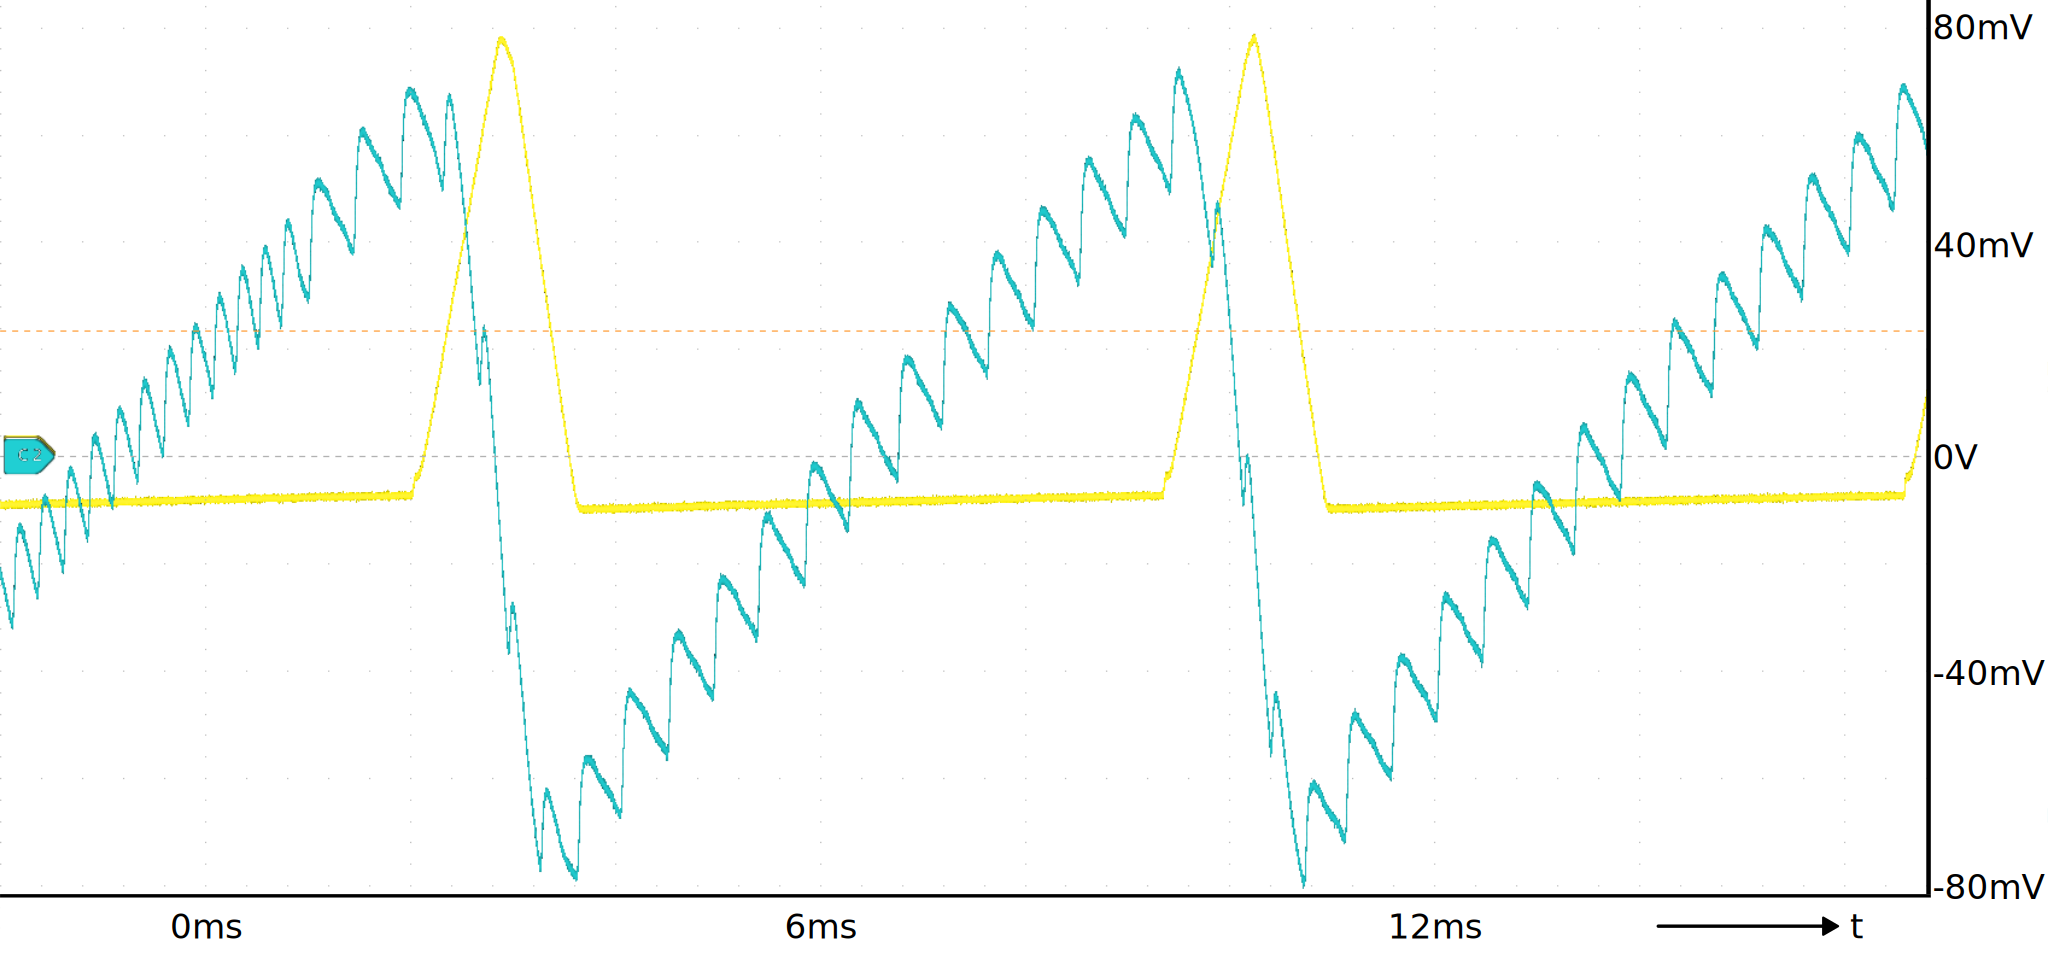
\includegraphics[scale=0.17]{testUgsUds.png}\\
\end{frame}

\begin{frame}
    \frametitle{pH 7 Test}
    \centering
    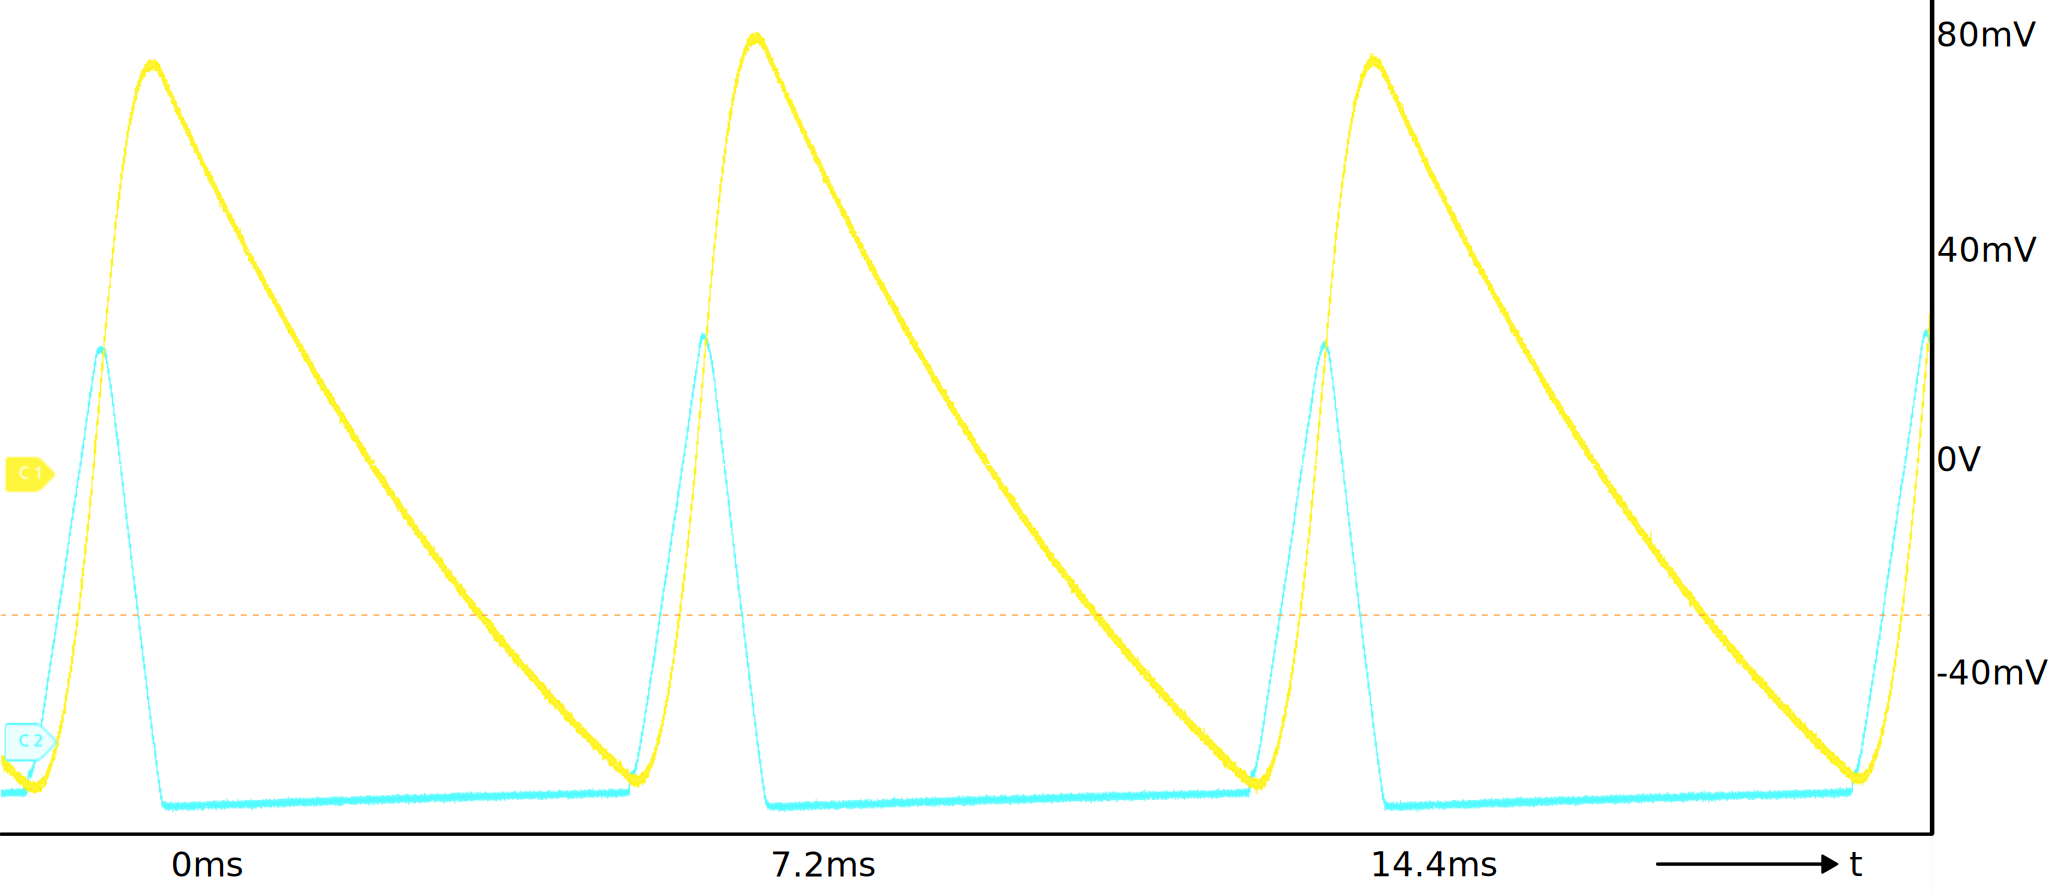
\includegraphics[scale=0.17]{testpH7.png}\\
\end{frame}

\begin{frame}
    \frametitle{pH 4 Test}
    \centering
    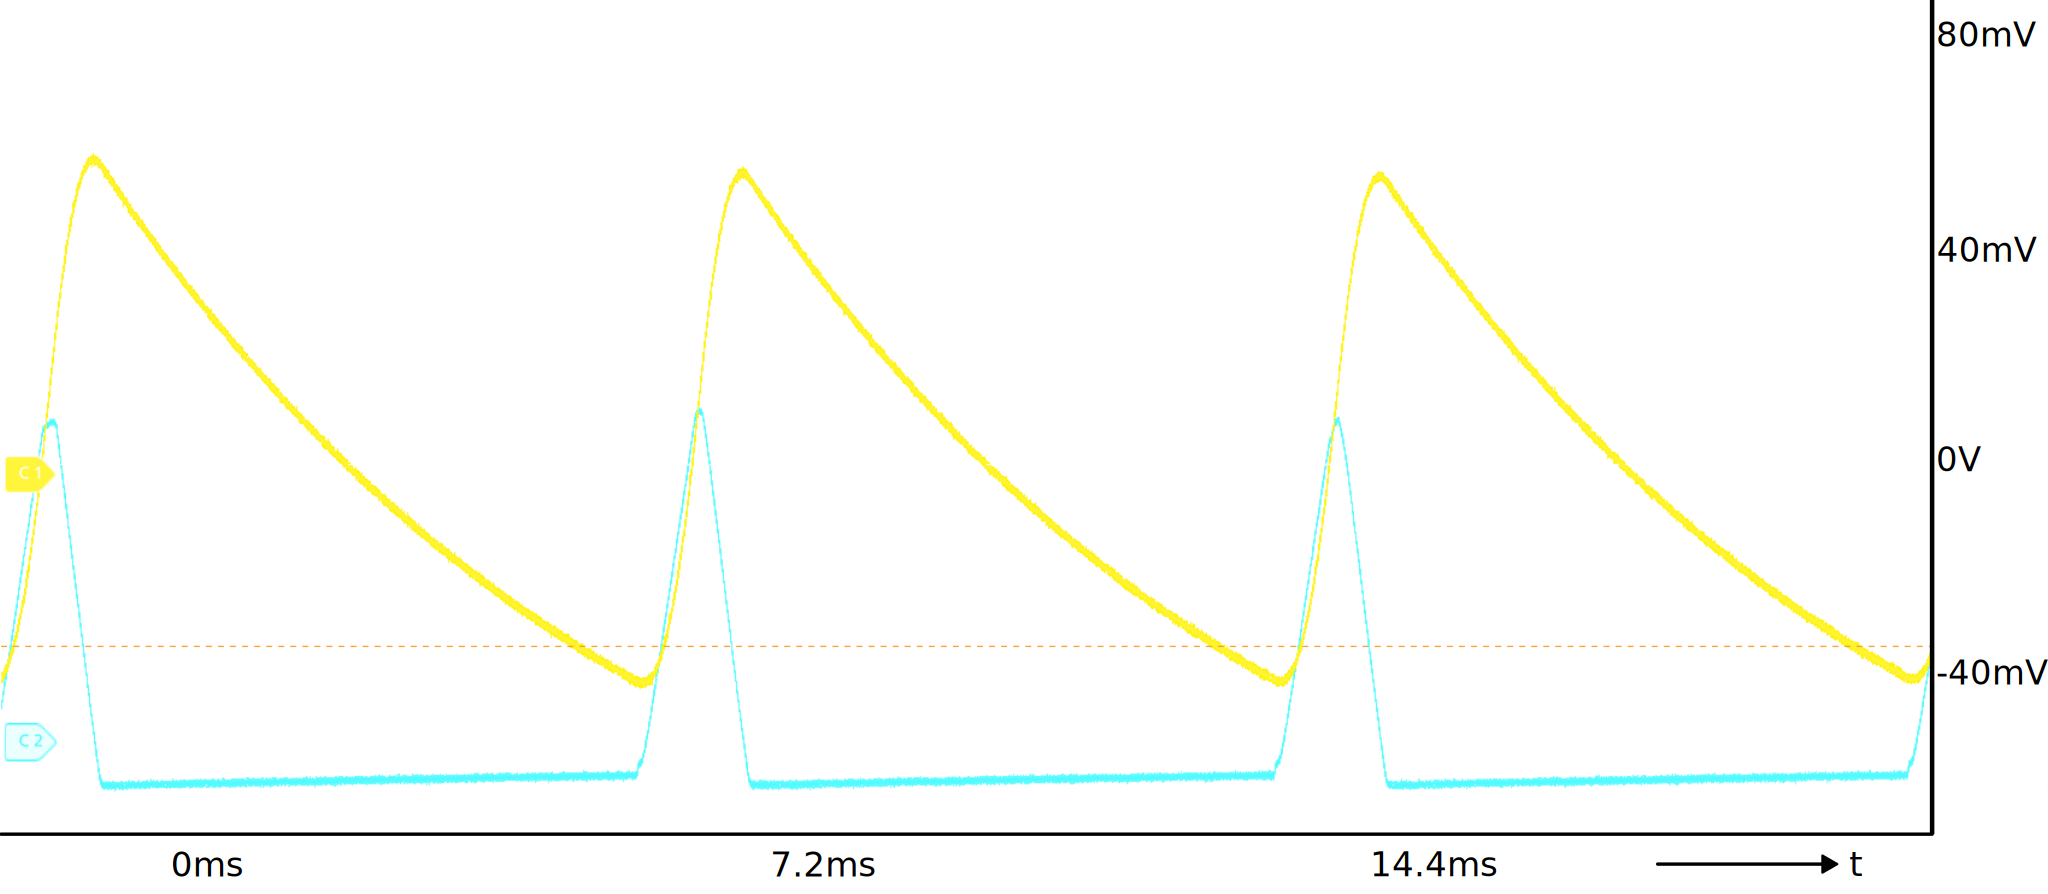
\includegraphics[scale=0.17]{testpH4.png}\\
\end{frame}

\begin{frame}
    \frametitle{Enervery harvesting test opstelling}
    \centering
    \includegraphics[scale=0.4]{energyHarvestingOpstelling.png}\\
\end{frame}
